\documentclass{article}
\usepackage{graphicx}
\usepackage{float}
\usepackage{amsmath}
\usepackage{amsfonts}
\usepackage{amssymb}
\usepackage{hyperref}
\usepackage{esint}
\usepackage[utf8]{inputenc}
\usepackage[a4paper, portrait, margin=0.75in]{geometry}
\setlength\parindent{0pt}
\usepackage[italian]{babel}
\usepackage{blindtext}

\usepackage{wasysym}


\hypersetup{
    colorlinks=true,
    linkcolor=black,
    filecolor=magenta,
    urlcolor=blue,
    pdftitle={APPLICAZIONI INDUSTRIALI ELETTRICHE ED ELETTRONICA},
    pdfpagemode=FullScreen,
}


\begin{document}
    \author{dmotrio}
    \title{APPLICAZIONI INDUSTRIALI ELETTRICHE ED ELETTRONICA - teoria}
    \date{Marzo 2022}

    \maketitle
    \tableofcontents

    \listoffigures
    \listoftables

    \section{Introduzione}

Le grandezze principali sono la \textbf{tensione}(campo elettrico) e la \textbf{corrente}(campo magnetico).

\subsection{Tensione}

\begin{figure}[H]
    \centering
    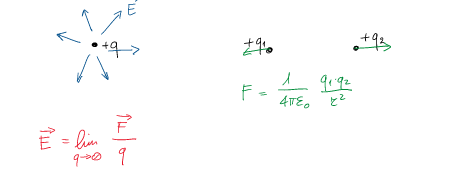
\includegraphics[width=0.7\linewidth]{imgs/tensione}
    \caption{tensione}
    \label{fig:tensione}
\end{figure}

La tensione V è:
\begin{equation}
    \vec{E} = - grad V = -\frac{\delta V}{\delta x} \hat{x}
    -\frac{\delta V}{\delta y} \hat{y}
    -\frac{\delta V}{\delta z} \hat{z}
\end{equation}

Detto anche potenziale elettrico, è l'energia potenziale elettrica normalizzata per la carica.

La tensione è la differenza di potenziale elettrico(d.d.p.).
\subsubsection{Unità di misura della tensione}
La tensione si misura in \textbf{volt} $[V]$.

\begin{itemize}
    \item $[q] = C$ "coulomb" $= A\cdot s$ "Ampere per secondo"
    \item $[E] = \frac{N}{C} = \frac{N}{A\cdot s} =
    \frac{Kg \cdot \frac{m}{s^2}}{A\cdot s}$
    \item $V = \frac{N\cdot m}{A \cdot s}$
\end{itemize}

Ricorda che la tensione dal punto B ad A si chiama $V_{AB}$ e che $V_{AB} = - V_{BA}$.










\end{document}